\part[Collections]{Collections}
\section{Overview of the Collections API}
\begin{frame}{Overview - Package Hierarchy}
\begin{center}
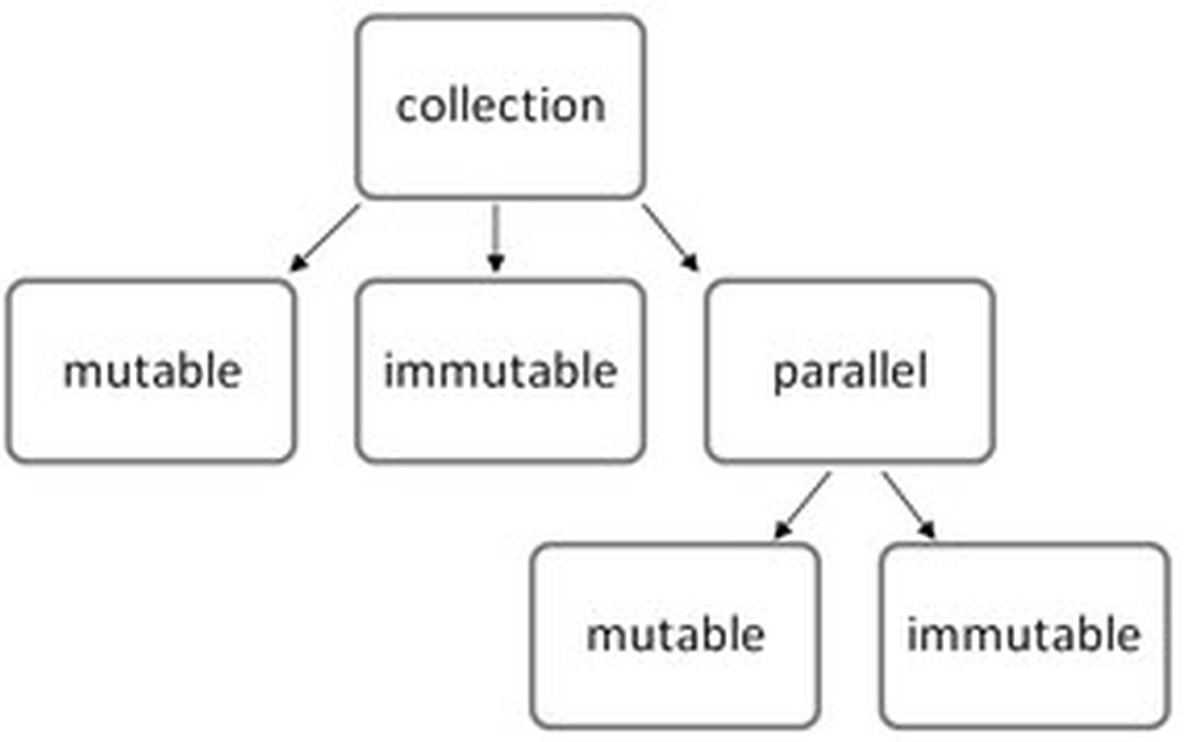
\includegraphics{resources/PackageHierarchy.jpg}
\end{center}
\end{frame}

\begin{frame}{Overview - Class Hierarchy}
\begin{center}
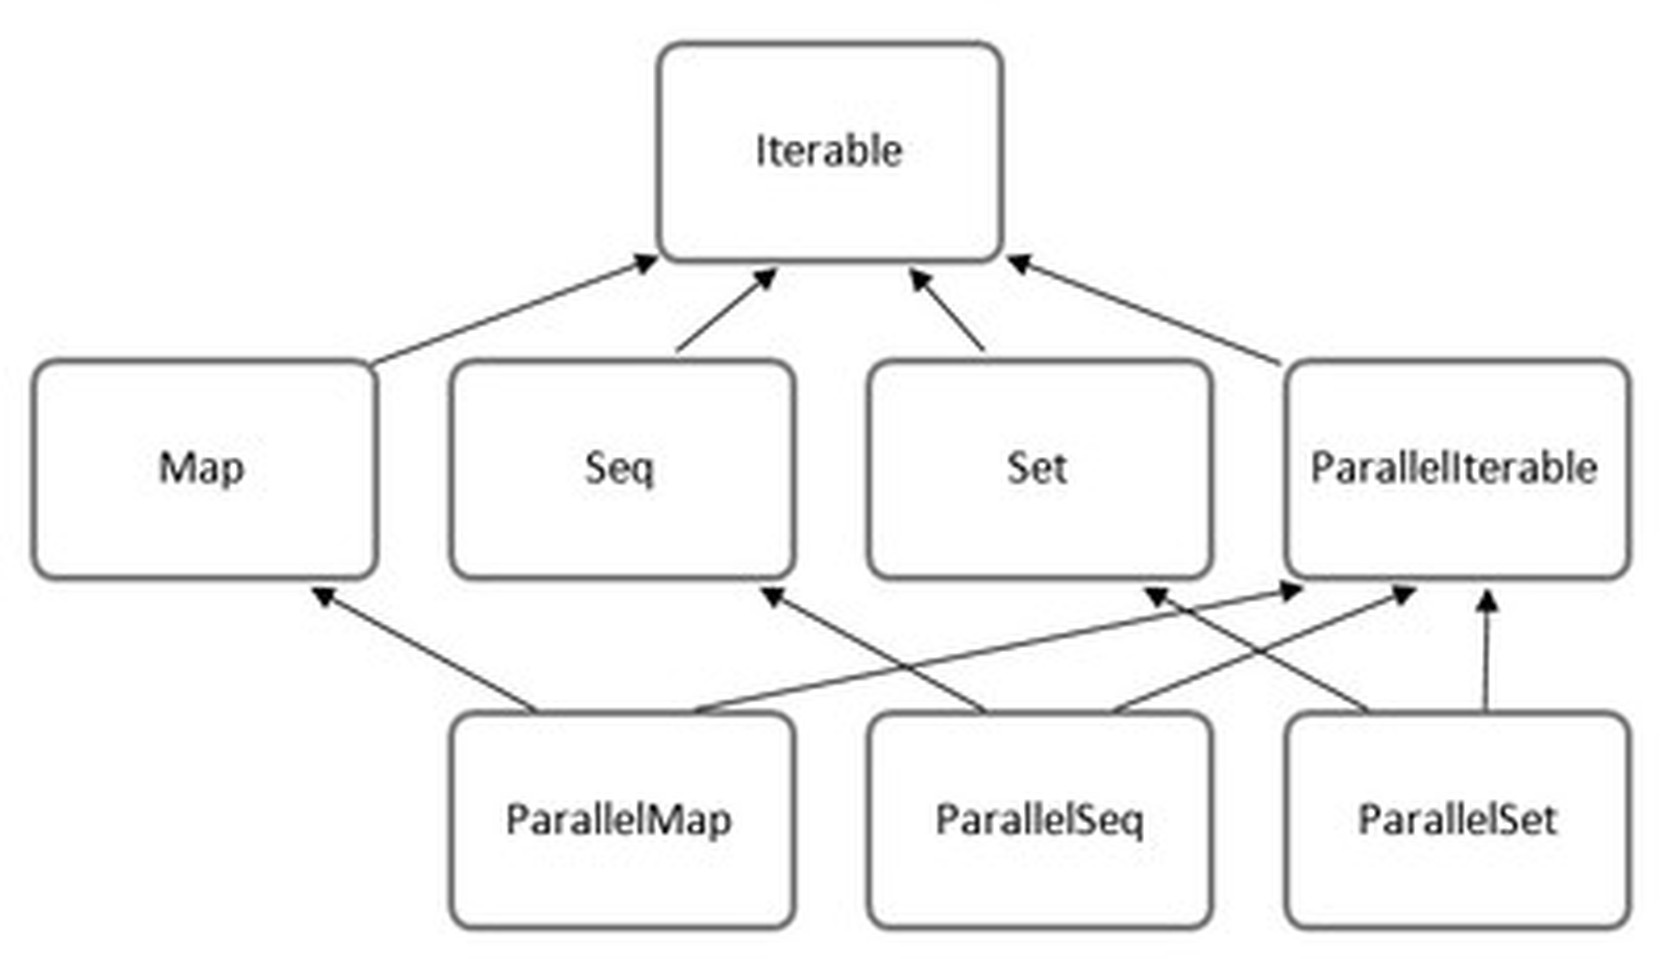
\includegraphics[width = 0.9\textwidth]{resources/ClassHierarchy.jpg}
\end{center}
\end{frame}

\begin{frame}{Overview - collection}
\begin{center}
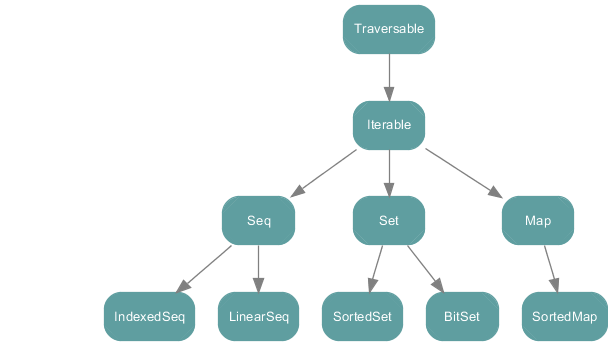
\includegraphics[width = \textwidth]{resources/collection.png}
\end{center}
\end{frame}

\begin{frame}{Overview - collection.immutable}
\begin{center}
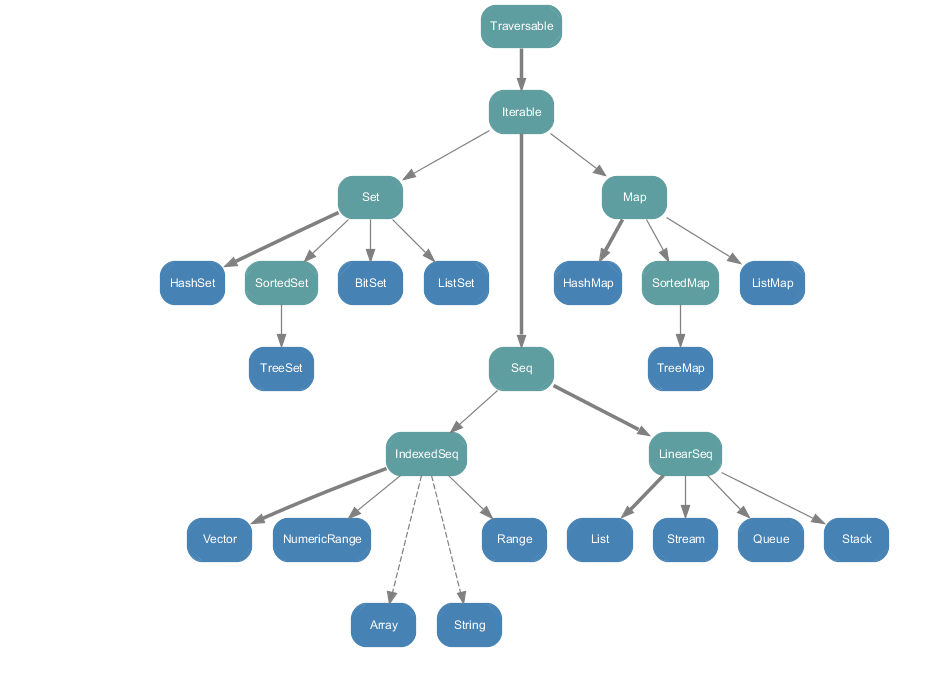
\includegraphics[width = \textwidth]{resources/collectionImmutable.png}
\end{center}
\end{frame}

\begin{frame}{Overview - collection.mutable}
\begin{center}
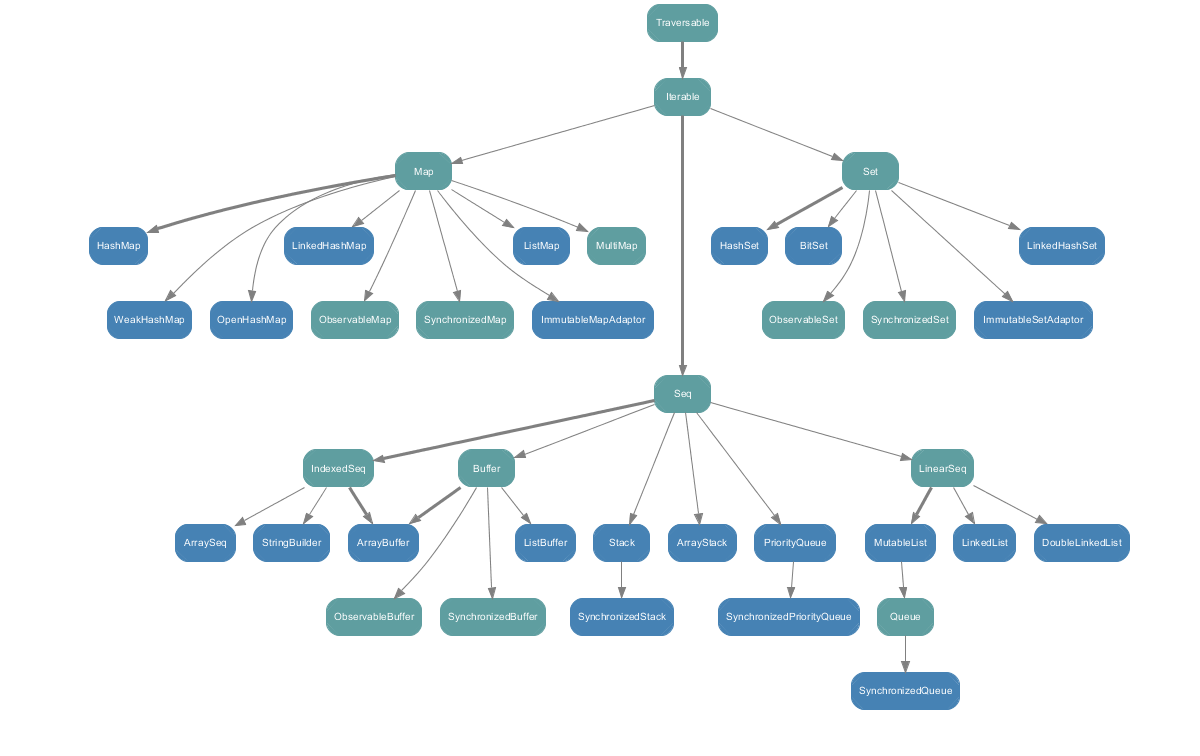
\includegraphics[width = \textwidth]{resources/collectionMutable.png}
\end{center}
\end{frame}

\begin{frame}{Overview - collection.parallel}
\begin{center}
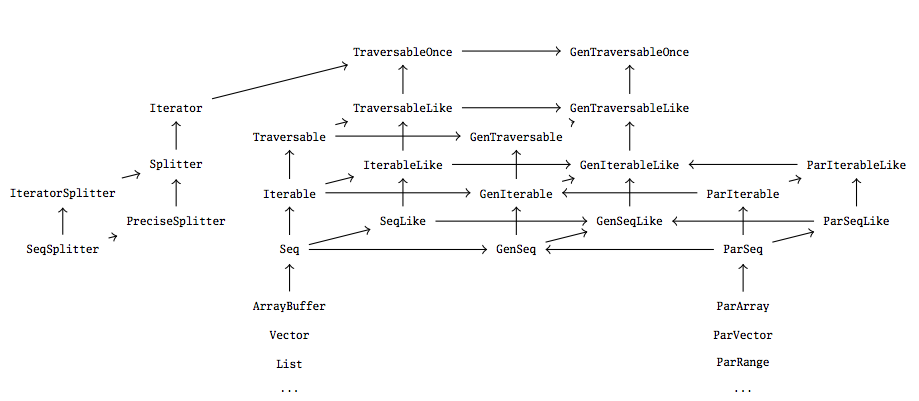
\includegraphics[width = \textwidth]{resources/collectionParallel.png}
\end{center}
\end{frame}

\begin{frame}[fragile]{Overview - Uniform syntax}
\begin{lstlisting}
Traversable(1, 2, 3)
Iterable("x", "y", "z")
Map("x" -> 24, "y" -> 25, "z" -> 26)
Set(Color.red, Color.green, Color.blue)
SortedSet("hello", "world")
Buffer(x, y, z)
IndexedSeq(1.0, 2.0)
LinearSeq(a, b, c) 
List(1, 2, 3)
HashMap("x" -> 24, "y" -> 25, "z" -> 26) 
\end{lstlisting}
\end{frame}

\begin{frame}[fragile]{Overview - Uniform return type principle}
\begin{lstlisting}
scala> List(1, 2, 3) map { _ + 1 }
res0: List[Int] = List(2, 3, 4)

scala> Set(1, 2, 3) map { _ + 1 }
res1: Set[Int] = Set(2, 3, 4) 
\end{lstlisting}
\end{frame}

\begin{frame}[fragile]{Overview - Type inference}
\begin{lstlisting}
import scala.collection.(im)mutable.HashMap

// no inference
val x: HashMap[String, Int] = new HashMap[String, Int]
val x: HashMap[String, Int] = HashMap[String, Int]()

// object inference
val x: HashMap[String, Int] = new HashMap
val x: HashMap[String, Int] = HashMap()

// reference inference
val x = new HashMap[String, Int]
val x = HashMap[String, Int]()

// full inference
val x = HashMap("dog" -> 3)
\end{lstlisting}
\end{frame}

\begin{frame}[fragile]{Overview - Trait Traversable}
\begin{center}
\lstinline!def foreach[U](f: Elem => U): Unit!
\end{center}
\begin{center}
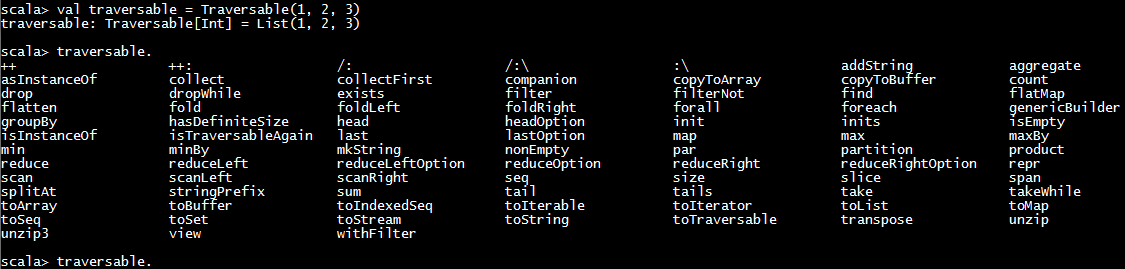
\includegraphics[width = \textwidth]{resources/Traversable.png}
\end{center}
\end{frame}

\begin{frame}[fragile]{Overview - Trait Iterable}
\begin{center}
\begin{lstlisting}
def foreach[U](f: Elem => U): Unit = {
  val it = iterator
  while (it.hasNext)
    f(it.next())
} 
\end{lstlisting}
\end{center}
\begin{center}
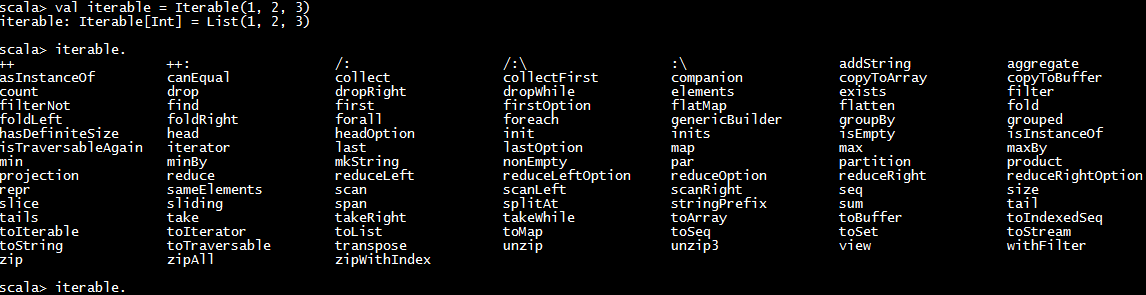
\includegraphics[width = \textwidth]{resources/Iterable.png}
\end{center}
\end{frame}

\begin{frame}[fragile]{Overview - Trait Iterable}
\begin{exampleblock}{grouped}
\begin{lstlisting}
scala> val xs = List(1, 2, 3, 4, 5)
xs: List[Int] = List(1, 2, 3, 4, 5)

scala> val git = xs grouped 3
git: Iterator[List[Int]] = non-empty iterator

scala> git.next()
res0: List[Int] = List(1, 2, 3)

scala> git.next()
res1: List[Int] = List(4, 5)
\end{lstlisting}
\end{exampleblock}
\end{frame}

\begin{frame}[fragile]{Overview - Trait Iterable}
\begin{exampleblock}{sliding}
\begin{lstlisting}
scala> val xs = List(1, 2, 3, 4, 5)
xs: List[Int] = List(1, 2, 3, 4, 5)

scala> val sit = xs sliding 3
sit: Iterator[List[Int]] = non-empty iterator

scala> sit.next()
res0: List[Int] = List(1, 2, 3)

scala> sit.next()
res1: List[Int] = List(2, 3, 4)

scala> sit.next()
res2: List[Int] = List(3, 4, 5) 
\end{lstlisting}
\end{exampleblock}
\end{frame}

\begin{frame}[fragile]{Overview - Seq, Set and Map}
\begin{exampleblock}{apply}
\begin{lstlisting}
scala> val seq = Seq(1, 2, 3)
seq: Seq[Int] = List(1, 2, 3)

scala> seq(1)
res0: Int = 2

scala> val set = Set(1, 2, 3)
set: Set[Int] = Set(1, 2, 3)

scala> set(1)
res1: Boolean = true

scala> val map = Map(1 -> "I", 2 -> "II", 3 -> "III")
map: Map[Int, java.lang.String] = Map(1 -> I, 2 -> II, 3 -> III)

scala> map(1)
res2: java.lang.String = I
\end{lstlisting}
\end{exampleblock}
\end{frame}

\begin{frame}[fragile]{Overview - Seq, IndexedSeq and LinearSeq}
The \lstinline!Seq trait! represents sequences. A \lstinline!Seq! is a kind of
\lstinline!Iterable! that has a \highlight{length} and whose elements have
\highlight{fixed index positions}, starting from 0.\\
\begin{center}
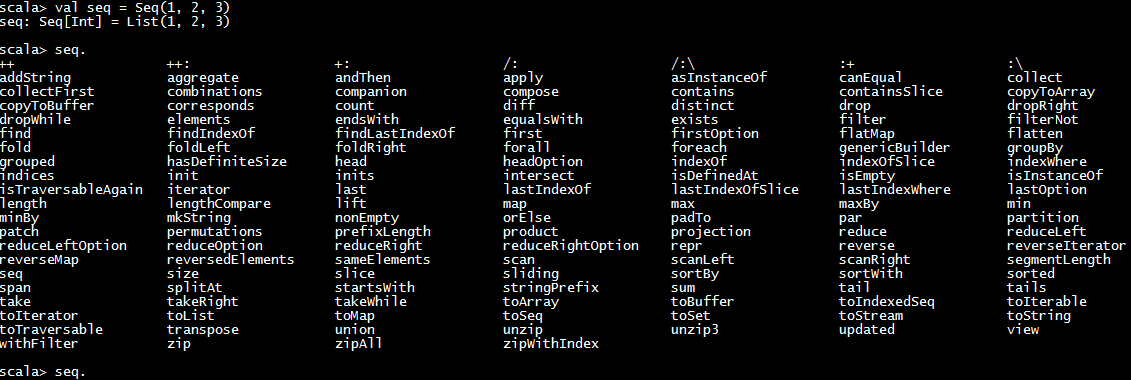
\includegraphics[width = \textwidth]{resources/Seq.png}
\end{center}
\end{frame}

\begin{frame}[fragile]{Overview - Seq, IndexedSeq and LinearSeq}
Trait \lstinline!Seq! has two subtraits: \lstinline!LinearSeq! and
\lstinline!IndexedSeq!. These do not add any new operations, but each offers
different performance characteristics: A linear sequence has efficient
\highlight{head and tail operations}, whereas an indexed sequence has efficient
\highlight{apply, length, and (if mutable) update operations}. Frequently used
linear sequences are \lstinline!immutable.List! and
\lstinline!immutable.Stream!. Frequently use  indexed sequences are
\lstinline!scala.Array! and \lstinline!mutable.ArrayBuffer!.
\newline
\newline
The \lstinline!Vector! class provides an interesting compromise between indexed
and linear access. It has \highlight{both effectively constant time indexing
overhead and constant time linear access overhead}. Because of this, vectors are
a good foundation for mixed access patterns where both indexed and linear
accesses are used.\\
\begin{center}
Use \lstinline!Vector! as your \highlight{default collection}
\end{center}
\end{frame}

\begin{frame}[fragile]{Overview - Sets}
\begin{center}
\lstinline!Set!s are \lstinline!Iterable!s that contain no duplicate elements
\end{center}
\begin{center}
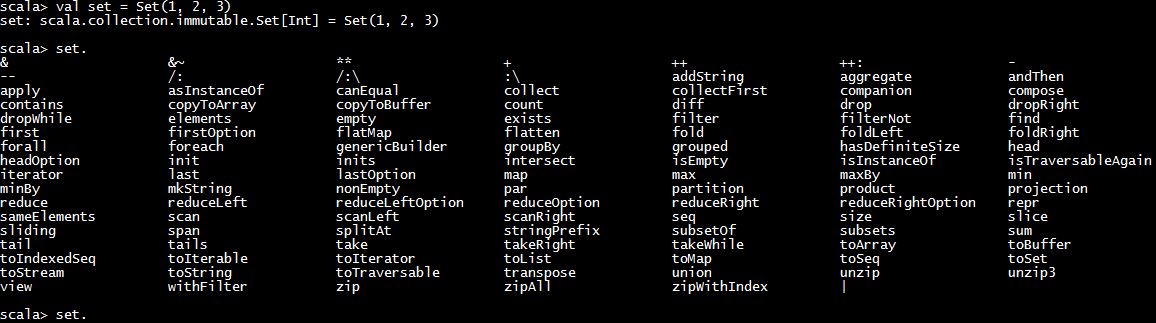
\includegraphics[width = \textwidth]{resources/Set.png}
\end{center}
\begin{lstlisting}
scala> val set = Set(1, 2, 3, 1, 2, 2, 4)
set: scala.collection.immutable.Set[Int] = Set(1, 2, 3, 4)
\end{lstlisting}
\end{frame}

\begin{frame}[fragile]{Overview - Maps}
A \lstinline!Map! is an \lstinline!Iterable! consisting of pairs of keys and
values (also named mappings or associations). Scala's \lstinline!Predef class!
offers an \highlight{implicit conversion} that lets you write \lstinline!key -> value! as
an alternate syntax for the pair \lstinline!(key, value)!.
\begin{center}
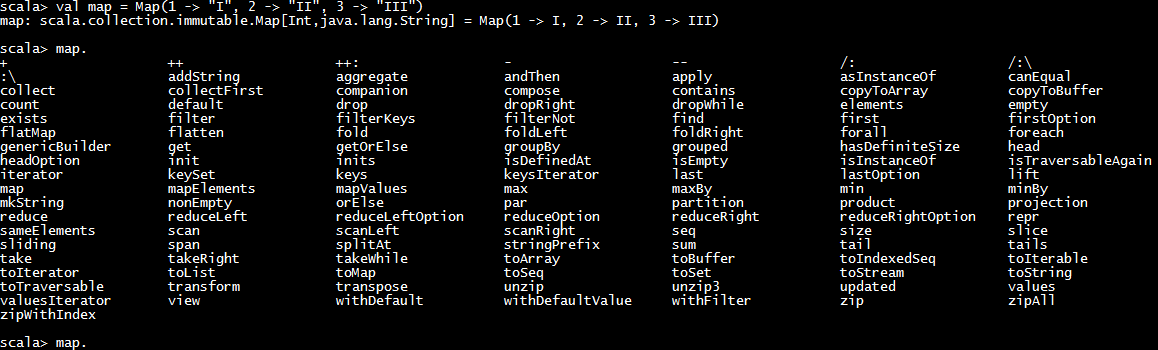
\includegraphics[width = \textwidth]{resources/Map.png}
\end{center}
\end{frame}

\section{Concrete Immutable Collection Classes}
\begin{frame}[fragile]{Streams}
A \lstinline!Stream! is like a \lstinline!List! except that its elements are
computed \lstinline!lazily!. Because of this, a stream can be
\lstinline!infinitely! long. Only those elements requested are computed.
Otherwise, streams have the same performance characteristics as lists.
\newline
\newline
Whereas lists are constructed with the \lstinline!::! operator, streams are
constructed with the similar-looking \lstinline!#::! operator. Here is a simple
example of a stream containing the integers 1, 2, and 3:\\
\begin{exampleblock}{\lstinline!Stream! - the lazy \lstinline!List!}
\begin{lstlisting}
scala> val str = 1 #:: 2 #:: 3 #:: Stream.empty
str: scala.collection.immutable.Stream[Int] = Stream(1, ?)
\end{lstlisting}
\end{exampleblock}
The head of this stream is 1, and the tail of it has 2 and 3. The tail is not
printed here, though, because it hasn't been computed yet! Streams are specified
to compute lazily, and the \lstinline!toString! method of a stream is careful
not to force any extra evaluation.
\end{frame}

\begin{frame}[fragile]{Streams}
\begin{exampleblock}{Infinite memory is overrated ;)}
\begin{lstlisting}
scala> val ones: Stream[Int] = 1 #:: ones
ones: Stream[Int] = Stream(1, ?)

scala> ones take 10 foreach print
1111111111
\end{lstlisting}
\end{exampleblock}
\pause
\begin{exampleblock}{How many Fibonacci implementations are there? ;)}
\begin{lstlisting}
scala> def fib(a: Int, b: Int): Stream[Int] = a #:: fib(b, a + b)
fib: (a: Int, b: Int)Stream[Int]

scala> val fibs = fib(1, 1) take 7 toList
fibs: List[Int] = List(1, 1, 2, 3, 5, 8, 13)
\end{lstlisting}
\end{exampleblock}
\end{frame}

\begin{frame}[fragile]{Vectors}
\begin{lstlisting}[belowskip=3mm]
scala> val vec = Vector(1, 2, 3)
vec: immutable.Vector[Int] = Vector(1, 2, 3)
\end{lstlisting}
\pause
\begin{lstlisting}[belowskip=3mm]
scala> val vec2 = vec :+ 4 :+ 5
vec2: immutable.Vector[Int] = Vector(1, 2, 3, 4, 5)
\end{lstlisting}
\pause
\begin{lstlisting}[belowskip=3mm]
scala> val vec3 = 0 +: vec2
vec3: immutable.Vector[Int] = Vector(0, 1, 2, 3, 4, 5)
\end{lstlisting}
\pause
\begin{lstlisting}[belowskip=3mm]
scala> val vec4 = vec3 updated (3, 6)
vec4: immutable.Vector[Int] = Vector(0, 1, 2, 6, 4, 5)
\end{lstlisting}
\pause
\begin{lstlisting}
scala> vec3(3)
res6: Int = 3

scala> vec4(3)
res7: Int = 6
\end{lstlisting}
\end{frame}

\begin{frame}[fragile]{Ranges}
\begin{center}
A \lstinline!Range! is an ordered sequence of integers that are \highlight{equally spaced apart}
\end{center}
\begin{lstlisting}[belowskip=3mm]
scala> val range = 1 to 3
range: immutable.Range.Inclusive = Range(1, 2, 3)

scala> val range = 1 until 3
range: immutable.Range = Range(1, 2)
\end{lstlisting}
\pause
\begin{lstlisting}
scala> val range = 1 to 10 by 3
range: immutable.Range = Range(1, 4, 7, 10)

scala> val range = 10 to 1 by -3
range: immutable.Range = Range(10, 7, 4, 1)
\end{lstlisting}
\end{frame}

\section{Performance Characteristics}
\begin{frame}{Performance characteristics}
\begin{center}
\begin{tabular}{|l|p{0.9\textwidth}|}
\hline
C & Constant time\\
\hline
eC & Effectively constant time, but this might depend on some assumptions such
as maximum length of a vector or distribution of hash keys.\\
\hline
aC & Amortized constant time. Some invocations might take longer, but if many
operations are performed on average only constant time per operation is taken.\\
\hline
Log & Time proportional to the logarithm of the collection size.\\
\hline
L & Linear time proportional to the collection size.\\
\hline
- & The operation is not supported.\\
\hline
\end{tabular}
\end{center}
\end{frame}
\begin{frame}{Performance characteristics of sequence types}
\begin{tabular}{|l|l|l|l|l|l|l|l|}
\hline
& head & tail & apply & update & prepend & append & insert\\
\hline
\highlight{immutable}\\
\hline
List & C & C & L & L & C & L & -\\
\hline
Stream & C & C & L & L & C & L & -\\
\hline
Vector & eC & eC & eC & eC & eC & eC & -\\
\hline
Stack & C & C & L & L & C & L & -\\
\hline
Queue & aC & aC & L & L & L & C & -\\
\hline
Range & C & C & C & - & - & - & -\\
\hline
String & C & L & C & L & L & L & -\\
\hline
\end{tabular}
\end{frame}

\begin{frame}{Performance characteristics of sequence types}
\begin{tabular}{|l|l|l|l|l|l|l|l|}
\hline
& head & tail & apply & update & prepend & append & insert\\
\hline
\highlight{mutable}\\
\hline
ArrayBuffer & C & L & C & C & L & aC & L\\
\hline
ListBuffer & C & L & L & L & C & C & L\\
\hline
StringBuilder & C & L & C & C & L & aC & L\\
\hline
MutableList & C & L & L & L & C & C & L\\
\hline
Queue & C & L & L & L & C & C & L\\
\hline
ArraySeq & C & L & C & C & - & - & -\\
\hline
Stack & C & L & L & L & C & L & L\\
\hline
ArrayStack & C & L & C & C & aC & L & L\\
\hline
Array & C & L & C & C & - & - & -\\
\hline
\end{tabular}
\end{frame}

\begin{frame}{Performance characteristics of set and map types}
\begin{tabular}{|l|l|l|l|l|}
\hline
& lookup & add & remove & min\\
\hline
\highlight{immutable}\\
\hline
HashSet/HashMap & eC & eC & eC & L\\
\hline
TreeSet/TreeMap & Log & Log & Log & Log\\
\hline
BitSet & C & L & L & eC\\
\hline
ListMap & L & L & L & L\\
\hline
\highlight{mutable}\\
\hline
HashSet/HashMap & eC & eC & eC & L\\
\hline
WeakHashMap & eC & eC & eC & L\\
\hline
BitSet & C & aC & C & eC\\
\hline
\end{tabular}
\end{frame}

\section{Views}
\begin{frame}[fragile]{Views - Transformers}
\begin{block}{What is a transformer?}
A transformer is a higher-order method, which takes a collection as it's
argument (or simply put, a method, which is defined on a collection) and a
lambda and produces another collection as it's result, thus transforming the
input collection into the output one. E.g: \lstinline!map! or
\lstinline!filter!.
\end{block}
\pause
\begin{block}{Transformer implementations}
There are two principal ways to implement transformers:\\
\begin{description}
  \item[strict] - a new collection with all its elements is constructed as a
  result of the transformer
  \item[lazy] - one constructs only a proxy for the result collection, and its
  elements get constructed only as one demands them
\end{description}
\end{block}
\end{frame}

\begin{frame}[fragile]{Views - Transformers}
\begin{exampleblock}{Example of a non-strict \lstinline!map! method
(procedural notation)}
\begin{lstlisting}
def map[T, U](coll: Iterable[T], f: T => U) = new Iterable[T] {
  def iterator = coll.iterator map f
} 
\end{lstlisting}
\end{exampleblock}
\pause
\begin{exampleblock}{Example of a non-strict \lstinline!map! method (OO
notation)}
\begin{lstlisting}
class Iterable[+T] {
  def map[U](f: T => U) = new Iterable[T] {
    def iterator = this.iterator map f
  } 
}
\end{lstlisting}
\end{exampleblock}
\end{frame}

\begin{frame}[fragile]{Views - Switching back and forth}
\begin{block}{Default implementation}
Scala collections are by \highlight{default strict} in all their transformers,
\alert{except for Stream}, which implements all its transformer methods lazily.
However, there is a systematic way to turn every collection into a lazy one and
vice versa, which is based on collection views.
\end{block}
\pause
\begin{block}{What is a view?}
A \highlight{view} is a special kind of collection that represents some base
collection, but \highlight{implements all transformers lazily}.
\end{block}
\pause
\begin{block}{\lstinline!view! and \lstinline!force!}
To go from a collection to its view, you can use the \lstinline!view! method on
the collection. If \lstinline!xs! is some collection, then \lstinline!xs.view!
is the same collection, but with all transformers implemented lazily. To get
back from a view to a strict collection, you can use the \lstinline!force!
method.
\end{block}
\end{frame}

\begin{frame}[fragile]{Views - problem with strict transformers}
\begin{alertblock}{Mapping two functions in succession over a \lstinline!Vector[Int]!}
\begin{lstlisting}
scala> val vector = Vector(1, 2, 3)
vector: immutable.Vector[Int] = Vector(1, 2, 3)

scala> val modifiedVector = vector map { _ + 1 } map { _ * 2 }
modifiedVector: immutable.Vector[Int] = Vector(4, 6, 8)
\end{lstlisting}
\end{alertblock}
\pause
\begin{alertblock}{Mapping two functions in succession over a \lstinline!Vector[Int]!}
Performance issues, because additional vectors are created for each \lstinline!map! invocation.
\end{alertblock}
\end{frame}

\begin{frame}[fragile]{Views - solution for strict transformers I}
\begin{exampleblock}{Single map with the composition of \lstinline!(_ + 1)! and \lstinline!(_ * 2)!}
\begin{lstlisting}
scala> val modifiedVector = vector map { x => (x + 1) * 2}
modifiedVector: immutable.Vector[Int] = Vector(4, 6, 8)
\end{lstlisting}
\end{exampleblock}
\begin{exampleblock}{Single map with the composition of \lstinline!(_ + 1)! and \lstinline!(_ * 2)!}
\begin{lstlisting}
scala> val modifiedVector = vector map { 
     |    ((_: Int) + 1) andThen (_ * 2)
     | }
modifiedVector: immutable.Vector[Int] = Vector(4, 6, 8)
\end{lstlisting}
\end{exampleblock}
\end{frame}

\begin{frame}[fragile]{Views - solution for strict transformers II}
\begin{exampleblock}{vector to view to vector}
\begin{lstlisting}
scala> val v = (vector.view map { _ + 1 } map {_ * 2}).force
v: immutable.Vector[Int] = Vector(4, 6, 8)
\end{lstlisting}
\end{exampleblock}
\pause
\begin{exampleblock}{vector to view to vector step by step}
\begin{lstlisting}[belowskip=3mm]
scala> val vv = vector.view
vv: java.lang.Object with
scala.collection.SeqView[Int,immutable.Vector[Int]] = SeqView(...)
\end{lstlisting}
\pause
\begin{lstlisting}[belowskip=3mm]
scala> val vvm = vv map { _ + 1 }
vvm: scala.collection.SeqView[Int,Seq[_]] = SeqViewM(...)
\end{lstlisting}
\pause
\begin{lstlisting}[belowskip=3mm]
scala> val vvmm = vvm map { _ * 2 }
vvmm: scala.collection.SeqView[Int,Seq[_]] = SeqViewMM(...)
\end{lstlisting}
\pause
\begin{lstlisting}[belowskip=3mm]
scala> val v = vvmm.force
v: Seq[Int] = Vector(4, 6, 8)
\end{lstlisting}
\end{exampleblock}
\end{frame}

\begin{frame}[fragile]{Views - another example}
\begin{block}{Finding the first palindrome in a list of words}
\begin{lstlisting}
def isPalindrome(x: String) = x == x.reverse
def findPalidrome(s: Seq[String]) = s find isPalindrome 
\end{lstlisting}
\end{block}
\pause
\begin{center}
Finding the first palindrome in the first million words of a \alert{VERY long} sequence
\end{center}
\pause
\begin{alertblock}{What is the problem?}
\lstinline!findPalindrome(words take 1000000)!
\end{alertblock}
\pause
\begin{exampleblock}{No superfluous construction of new sequences}
\lstinline!findPalindrome(words.view take 1000000)!
\end{exampleblock}
\end{frame}

\section{Parallel Collections}
\begin{frame}{Parallel Collections}
The idea is simple � collections are a well-understood and frequently-used
programming abstraction. And given their regularity, they're able to be
efficiently parallelized, transparently. By allowing a user to \highlight{``swap
out''} sequential collections for ones that are operated on in parallel, Scala's
parallel collections take a large step forward in enabling parallelism to be
easily brought into more code
\end{frame}

\begin{frame}[fragile]{Parallel Collections - Overview}
The design of Scala's parallel collections library is inspired by and deeply
integrated with Scala's (sequential) collections library (introduced in 2.8). It
provides a \highlight{parallel counterpart} to a number of important data
structures from Scala�s (sequential) collection library, including:
\begin{itemize}
  \item ParArray
  \item ParVector
  \item (im)mutable.ParHashMap
  \item (im)mutable.ParHashSet
  \item ParRange
  \item ParTrieMap (collection.concurrent.TrieMaps are new in 2.10)
\end{itemize}
\end{frame}

\begin{frame}[fragile]{Parallel Collections - Creation}
\begin{lstlisting}
scala> import scala.collection.parallel
import scala.collection.parallel

scala> mutable.ParArray(1, 2, 3)
res0: parallel.mutable.ParArray[Int]
= ParArray(1, 2, 3)

scala> immutable.ParVector(1, 2, 3)
res1: scala.collection.parallel.immutable.ParVector[Int]
= ParVector(1, 2, 3)

scala> immutable.ParHashMap(1 -> "I", 2 -> "II")
res2: scala.collection.parallel.immutable.ParHashMap[Int,String]
= ParMap(1 -> I, 2 -> II)

scala> mutable.ParHashSet(1 -> "I", 1 -> "I")
res3: scala.collection.parallel.mutable.ParHashSet[(Int, String)]
= ParHashSet((1,I))
\end{lstlisting}
\end{frame}

\begin{frame}[fragile]{Parallel Collections - Swaping back and forth}
\begin{lstlisting}
scala> val sequentialList = (1 to 1000000).toList
sequentialList: List[Int] = List(1, 2, 3, ... , 999999, 1000000)

scala> val parallelList = sequentialList.par 
parallelList: scala.collection.parallel.immutable.ParSeq[Int]
= ParVector(1, 2, 3, ... , 999999, 1000000)

scala> val sequentialList = parallelList.seq
sequentialList: scala.collection.immutable.Seq[Int]
= Vector(1, 2, 3, ... , 999999, 1000000)
\end{lstlisting}
\end{frame}

\begin{frame}[fragile]{Parallel Collections - Swaping back and forth}
\begin{block}{Implicit parallelism - Meaning}
From now on, every operation like e.g. \lstinline!map! is executed in parallel
\end{block}
\pause
\begin{exampleblock}{Implicit parallelism - Same API}
\begin{lstlisting}
sequentialList map { _ + 1 }
parallelList map { _ + 1 }
\end{lstlisting}
\end{exampleblock}
\pause
\begin{block}{Implicit parallelism - Rules}
The \lstinline!.par! invocation constructs a parallel collection, where
\highlight{the order} of the sequential input collection (if any) \highlight{is
preserved}, but the first-class function itself is executed \alert{without} any
particular \alert{order}.
\end{block}
\pause
\begin{exampleblock}{Implicit parallelism - Order}
\begin{lstlisting}
List(1,2,3).par foreach print // could print out 213
\end{lstlisting}
\end{exampleblock}
\end{frame}

\begin{frame}[fragile]{Parallel Collections != Concurrent Collections!}
\begin{alertblock}{Welcome back to the land of dead locks and starvation}
\begin{lstlisting}
scala> var sum = 0
sum: Int = 0

scala> parallelList foreach { sum += _ }

scala> println(sum)
-1471040024

scala> sum = 0
sum: Int = 0

scala> parallelList foreach { sum += _ }

scala> println(sum)
598796552
\end{lstlisting}
\end{alertblock}
\end{frame}

\begin{frame}[fragile]{Parallel Collections != Concurrent Collections!}
\begin{alertblock}{Welcome back to the land of dead locks and starvation}
\begin{lstlisting}
scala> @volatile var sum = 0
sum: Int = 0

scala> parallelList foreach { sum += _ }

scala> println(sum)
-1979434583

scala> sum = 0
sum: Int = 0

scala> parallelList foreach { sum += _ }

scala> println(sum)
1828316619
\end{lstlisting}
\end{alertblock}
\end{frame}

\begin{frame}[fragile]{Parallel Collections != Concurrent Collections!}
\begin{exampleblock}{No side effects}
\begin{lstlisting}
scala> val sum = parallelList reduceLeft { _ + _ }
sum: Int = 1784293664

scala> val sum = parallelList reduceLeft { _ + _ }
sum: Int = 1784293664

scala> val sum = parallelList reduceLeft { _ + _ }
sum: Int = 1784293664
\end{lstlisting}
\end{exampleblock}
\begin{exampleblock}{Common functions are already in the API}
\begin{lstlisting}
scala> val sum = parallelList.sum
sum: Int = 1784293664
\end{lstlisting}
\end{exampleblock}
\end{frame}

\section{Folding}
\begin{frame}[fragile]{Folds are functional loops}
\begin{block}{Loop}
\begin{lstlisting}
def sum(numbers: Seq[Int]) = {
  var result = 0
  var index = 0
  while(index < numbers.length) {
    val current = numbers(index)
    result += current
    index += 1
  }
  result
}
\end{lstlisting}
\end{block}
\begin{exampleblock}{Fold}
\begin{lstlisting}
def sum(numbers: Seq[Int]) = numbers.foldLeft(0) {
   (result, current) => result + current
}
\end{lstlisting}
\end{exampleblock}
\end{frame}

\begin{frame}[fragile]{Folds are functional loops}
\begin{block}{Loop}
\begin{lstlisting}
def makeString(numbers: List[Int]) = {
  var result = numbers.head.toString
  var tail = numbers.tail
  while(tail != Nil) {
    val current = tail.head
    result += " " + current
    tail = tail.tail
  }
  result
}
\end{lstlisting}
\end{block}
\begin{exampleblock}{Fold}
\begin{lstlisting}
def makeString(numbers: Seq[Int]) = 
  numbers.tail.foldLeft(numbers.head.toString) {
    (result, current) => result + " " + current
  }
\end{lstlisting}
\end{exampleblock}
\end{frame}

\begin{frame}[fragile]{Reduce is a fold where the first element is a seed}
\begin{exampleblock}{Fold}
\begin{lstlisting}
def sum(numbers: Seq[Int]) = numbers.foldLeft(0) {
   (result, current) => result + current
}
\end{lstlisting}
\end{exampleblock}
\begin{exampleblock}{Reduce}
\begin{lstlisting}
def sum(numbers: Seq[Int]) = numbers.reduceLeft {
   (result, current) => result + current
}
\end{lstlisting}
\end{exampleblock}
\end{frame}

\begin{frame}[fragile]{Sum and Product}
\begin{exampleblock}{Sum}
\begin{lstlisting}
val sum = List(1, 2, 3).foldLeft(0) { _ + _ }
val sum = List(1, 2, 3).reduceLeft { _ + _ }
val sum = List(1, 2, 3).sum
\end{lstlisting}
\end{exampleblock}
\begin{exampleblock}{Product}
\begin{lstlisting}
val product = List(1, 2, 3).foldLeft(1) { _ * _ }
val product = List(1, 2, 3).reduceLeft { _ * _ }
val product = List(1, 2, 3).product
\end{lstlisting}
\end{exampleblock}
\end{frame}

\begin{frame}[fragile]{fold vs foldLeft vs foldRight}
\begin{exampleblock}{\lstinline!fold!}
\begin{lstlisting}
def fold[A1 >: A](z: A1)(op: (A1, A1) => A1): A1
// Folds the elements of this list
// using the specified associative binary operator.
\end{lstlisting}
\end{exampleblock}
\begin{exampleblock}{\lstinline!foldLeft! (tail-recursive)}
\begin{lstlisting}
def foldLeft[B](z: B)(f: (B, A) => B): B
// Applies a binary operator to a start value
// and all elements of this list, going left to right.
\end{lstlisting}
\end{exampleblock}
\begin{exampleblock}{\lstinline!foldRight!}
\begin{lstlisting}
def foldRight[B](z: B)(f: (A, B) => B): B 
// Applies a binary operator to all elements of this list
// and a start value, going right to left.
\end{lstlisting}
\end{exampleblock}
\end{frame}

\begin{frame}[fragile]{reduce vs reduceLeft vs reduceRight vs\ldots}
\begin{lstlisting}
def reduce[A1 >: A](op: (A1, A1) => A1): A1
def reduceLeft[B >: A](f: (B, A) => B): B
def reduceRight[B >: A](op: (A, B) => B): B
def reduceOption[A1 >: A](op: (A1, A1) => A1): Option[A1]
def reduceLeftOption[B >: A](op: (B, A) => B): Option[B]
def reduceRightOption[B >: A](op: (A, B) => B): Option[B] 
\end{lstlisting}
\begin{center}
In comparison to folding, the result type \lstinline!B! of reducing is even more
constrained to be the supertype of the element type \lstinline!A!
\end{center}
\end{frame}

\begin{frame}{Furhter Readings}
\begin{center}
\link{http://oldfashionedsoftware.com/2009/07/10/scala-code-review-foldleft-and-foldright/}{Folding}
\end{center}
\begin{center}
\link{http://oldfashionedsoftware.com/2009/07/30/lots-and-lots-of-foldleft-examples/}{Examples}
\end{center}
\end{frame}

\section{Monadic for Comprehensions}
\begin{frame}[fragile]{Monadic for Comprehensions}
\begin{block}{What are monadic methods?}
Monadic methods are a special kind of methods, which are usually used for
querying data sources
\end{block}
\pause
\begin{exampleblock}{Monadic methods}
\begin{lstlisting}
class List[+A] {
  def foreach[B](f: A => B): Unit
  def map[B](f: A => B): List[B]
  def flatMap[B](f: A => List[B]): List[B]
  def filter(p: A => Boolean): List[A]
}
\end{lstlisting}
\end{exampleblock}
\pause
\begin{block}{What is a monadic for comprehension?}
A for comprehension is \highlight{syntactic sugar} for monadic methods
\end{block}
\end{frame}

\begin{frame}[fragile]{Monadic for Comprehensions}
\begin{center}
\lstinline!case class Person(name: String, age: Int)!
\lstinline!val people = List(Person("John", 12), Person("Fred", 38))!
\end{center}
\begin{exampleblock}{\lstinline!foreach!}
\begin{lstlisting}
people foreach { p => println(p.name) }

people foreach { case Person(name, _) => println(name) }
\end{lstlisting}
\end{exampleblock}
\begin{exampleblock}{\lstinline!foreach!}
\begin{lstlisting}
for(p <- people)
  println(p.name)

for(Person(name, _) <- people)
  println(name)
\end{lstlisting}
\end{exampleblock}
\begin{center}
\lstinline!John!\\
\lstinline!Fred!
\end{center}
\end{frame}

\begin{frame}[fragile]{Monadic for Comprehensions}
\begin{center}
\lstinline!case class Person(name: String, age: Int)!
\lstinline!val people = List(Person("John", 12), Person("Fred", 38))!
\end{center}
\begin{exampleblock}{\lstinline!map!}
\begin{lstlisting}
people map { p => p.name }

people map { case Person(name, _) => name }
\end{lstlisting}
\end{exampleblock}
\begin{exampleblock}{\lstinline!map!}
\begin{lstlisting}
for(p <- people)
  yield p.name

for(Person(name, _) <- people)
  yield name
\end{lstlisting}
\end{exampleblock}
\begin{center}
\lstinline!List(John, Fred)!\\
\lstinline!!
\end{center}
\end{frame}

\begin{frame}[fragile]{Monadic for Comprehensions}
\begin{lstlisting}
case class Person(name: String, age: Int, spokenLanguages: String*)
val people = List(
Person("John", 12, "EN", "DE"), 
Person("Fred", 38, "EN", "FR"))
\end{lstlisting}
\begin{exampleblock}{\lstinline!flatMap! - map andThen flatten!}
\begin{lstlisting}
people flatMap { person =>
  person.spokenLanguages map { language =>
     person.name + " " + language } }
\end{lstlisting}
\end{exampleblock}
\begin{exampleblock}{\lstinline!flatMap! - map andThen flatten!}
\begin{lstlisting}
for {
  person <- people
  language <- person.spokenLanguages
} yield person.name + " " + language
\end{lstlisting}
\end{exampleblock}
\begin{center}
\lstinline!List(John EN, John DE, Fred EN, Fred FR)!
\end{center}
\end{frame}

\begin{frame}[fragile]{Monadic for Comprehensions}
\begin{lstlisting}
case class Person(name: String, age: Int, spokenLanguages: String*)
val people = List(
Person("John", 12, "EN", "DE"), 
Person("Fred", 38, "EN", "FR"))
\end{lstlisting}
\begin{exampleblock}{\lstinline!flatMap! with \lstinline!filter!}
\begin{lstlisting}
people flatMap { person =>
  person.spokenLanguages filter { _ == "DE" } map { language =>
     person.name + " " + language } }
\end{lstlisting}
\end{exampleblock}
\begin{exampleblock}{\lstinline!flatMap! with \lstinline!filter!}
\begin{lstlisting}
for {
  person <- people
  language <- person.spokenLanguages
  if language == "DE"
} yield person.name + " " + language
\end{lstlisting}
\end{exampleblock}
\begin{center}
\lstinline!List(John DE)!
\end{center}
\end{frame}

\begin{frame}[fragile]{Monadic for Comprehensions}
\begin{lstlisting}
case class Person(name: String, age: Int, spokenLanguages: String*)
val people = List(
Person("John", 12, "EN", "DE"), 
Person("Fred", 38, "EN", "FR"))
\end{lstlisting}
\begin{exampleblock}{\lstinline!flatMap! with definitions and \lstinline!filter!}
\begin{lstlisting}
people flatMap { person =>
  person.spokenLanguages filter { _ == "DE" } map { language =>
     person.name + " " + language } }
\end{lstlisting}
\end{exampleblock}
\begin{exampleblock}{\lstinline!flatMap! with definitions and \lstinline!filter!}
\begin{lstlisting}
for {
  person <- people
  languages = person.spokenLanguages
  language <- languages
  if language == "DE"
  result = person.name + " " + language
} yield result
\end{lstlisting}
\end{exampleblock}
\end{frame}

\begin{frame}[fragile]{Monadic for Comprehensions}
\begin{center}
\lstinline!case class Book(title: String, authors: String*)!
\end{center}
\begin{exampleblock}{Book database}
\begin{lstlisting}
val books: List[Book] =
  List(
    Book("Structure and Interpretation of Computer Programs",
         "Abelson, Harold", "Sussman, Gerald J."),
    Book("Principles of Compiler Design",
         "Aho, Alfred", "Ullman, Jeffrey"),
    Book("Programming in Modula2",
         "Wirth, Niklaus"),
    Book("Elements of ML Programming",
         "Ullman, Jeffrey"),
    Book("The Java Language Specification", "Gosling, James",
         "Joy, Bill", "Steele, Guy", "Bracha, Gilad"))
\end{lstlisting}
\end{exampleblock}
\end{frame}

\begin{frame}[fragile]{Monadic for Comprehensions}
\begin{exampleblock}{Find all authors who have published at least two books}
\begin{lstlisting}
books flatMap (b1 =>
  books filter (b2 => b1 != b2) flatMap (b2 =>
    b1.authors flatMap (a1 =>
      b2.authors filter (a2 => a1 == a2) map (a2 => a1))))
\end{lstlisting}
\end{exampleblock}
\begin{exampleblock}{Find all authors who have published at least two books}
\begin{lstlisting}
for {
  b1 <- books
  b2 <- books
  if b1 != b2
  a1 <- b1.authors
  a2 <- b2.authors 
  if a1 == a2
} yield a1
\end{lstlisting}
\end{exampleblock}
\begin{center}
\lstinline!List(Ullman, Jeffrey, Ullman, Jeffrey)!
\end{center}
\end{frame}

\section{Summary}
\begin{frame}{Summary}
\begin{itemize}
  \item Scala's collection API is very mature
  \item The API has \highlight{immutable} and \highlight{mutable} collections
  \item The API has \highlight{sequential} and \highlight{parallel} collections
  \item The API has \highlight{strict} and {non-strict/lazy} collections
  \item The API lets you \highlight{convert} from seq to par collections and vice versa
  \item The API lets you \highlight{convert} from strict to lazy collections and vice versa
  \item Monadic \highlight{for comprehensions} let you query data sources in a highly readable manner
\end{itemize}
\end{frame}